\documentclass[11pt]{article}
\renewcommand{\arraystretch}{1.5} % Default value: 1
\usepackage{sectsty}
\allsectionsfont{\color{blue}\fontfamily{lmss}\selectfont}
\usepackage{fontspec}
\setmainfont{XCharter}

\usepackage{listings}
\lstset{
basicstyle=\small\ttfamily,
tabsize=8,
columns=flexible,
breaklines=true,
frame=tb,
rulecolor=\color[rgb]{0.8,0.8,0.7},
backgroundcolor=\color[rgb]{1,1,0.91},
postbreak=\raisebox{0ex}[0ex][0ex]{\ensuremath{\color{red}\hookrightarrow\space}}
}
\usepackage{fontawesome}


\usepackage{mdframed}
\newmdenv[
  backgroundcolor=gray,
  fontcolor=white,
  nobreak=true,
]{terminalinput}



\usepackage{parskip}
\usepackage{float}



    \usepackage[T1]{fontenc}
    % Nicer default font than Computer Modern for most use cases
    \usepackage{palatino}

    % Basic figure setup, for now with no caption control since it's done
    % automatically by Pandoc (which extracts ![](path) syntax from Markdown).
    \usepackage{graphicx}
    % We will generate all images so they have a width \maxwidth. This means
    % that they will get their normal width if they fit onto the page, but
    % are scaled down if they would overflow the margins.
    \makeatletter
    \def\maxwidth{\ifdim\Gin@nat@width>\linewidth\linewidth
    \else\Gin@nat@width\fi}
    \makeatother
    \let\Oldincludegraphics\includegraphics
    % Set max figure width to be 80% of text width, for now hardcoded.
\renewcommand{\includegraphics}[1]{\Oldincludegraphics[width=.8\maxwidth, height=.55\textheight, keepaspectratio]{#1}}
    % Ensure that by default, figures have no caption (until we provide a
    % proper Figure object with a Caption API and a way to capture that
    % in the conversion process - todo).
    \usepackage{caption}
    \DeclareCaptionLabelFormat{nolabel}{}
    \captionsetup{labelformat=nolabel, textfont=bf}

    \usepackage{adjustbox} % Used to constrain images to a maximum size
    \usepackage{xcolor} % Allow colors to be defined
    \usepackage{enumerate} % Needed for markdown enumerations to work
    \usepackage{geometry} % Used to adjust the document margins
    \usepackage{amsmath} % Equations
    \usepackage{amssymb} % Equations
    \usepackage{textcomp} % defines textquotesingle
    % Hack from http://tex.stackexchange.com/a/47451/13684:
    \AtBeginDocument{%
        \def\PYZsq{\textquotesingle}% Upright quotes in Pygmentized code
    }
    \usepackage{upquote} % Upright quotes for verbatim code
    \usepackage{eurosym} % defines \euro
    \usepackage[mathletters]{ucs} % Extended unicode (utf-8) support
    \usepackage[utf8x]{inputenc} % Allow utf-8 characters in the tex document
    \usepackage{fancyvrb} % verbatim replacement that allows latex
    \usepackage{grffile} % extends the file name processing of package graphics
                         % to support a larger range
    % The hyperref package gives us a pdf with properly built
    % internal navigation ('pdf bookmarks' for the table of contents,
    % internal cross-reference links, web links for URLs, etc.)
    \usepackage{hyperref}
    \usepackage{longtable} % longtable support required by pandoc >1.10
    \usepackage{booktabs}  % table support for pandoc > 1.12.2
    \usepackage[normalem]{ulem} % ulem is needed to support strikethroughs (\sout)
                                % normalem makes italics be italics, not underlines




    % Colors for the hyperref package
    \definecolor{urlcolor}{rgb}{0,.145,.698}
    \definecolor{linkcolor}{rgb}{.71,0.21,0.01}
    \definecolor{citecolor}{rgb}{.12,.54,.11}

    % ANSI colors
    \definecolor{ansi-black}{HTML}{3E424D}
    \definecolor{ansi-black-intense}{HTML}{282C36}
    \definecolor{ansi-red}{HTML}{E75C58}
    \definecolor{ansi-red-intense}{HTML}{B22B31}
    \definecolor{ansi-green}{HTML}{00A250}
    \definecolor{ansi-green-intense}{HTML}{007427}
    \definecolor{ansi-yellow}{HTML}{DDB62B}
    \definecolor{ansi-yellow-intense}{HTML}{B27D12}
    \definecolor{ansi-blue}{HTML}{208FFB}
    \definecolor{ansi-blue-intense}{HTML}{0065CA}
    \definecolor{ansi-magenta}{HTML}{D160C4}
    \definecolor{ansi-magenta-intense}{HTML}{A03196}
    \definecolor{ansi-cyan}{HTML}{60C6C8}
    \definecolor{ansi-cyan-intense}{HTML}{258F8F}
    \definecolor{ansi-white}{HTML}{C5C1B4}
    \definecolor{ansi-white-intense}{HTML}{A1A6B2}

    % commands and environments needed by pandoc snippets
    % extracted from the output of `pandoc -s`
    \providecommand{\tightlist}{%
      \setlength{\itemsep}{0pt}\setlength{\parskip}{0pt}}
    \DefineVerbatimEnvironment{Highlighting}{Verbatim}{commandchars=\\\{\}}
    % Add ',fontsize=\small' for more characters per line
    \newenvironment{Shaded}{}{}
    \newcommand{\KeywordTok}[1]{\textcolor[rgb]{0.00,0.44,0.13}{\textbf{{#1}}}}
    \newcommand{\DataTypeTok}[1]{\textcolor[rgb]{0.56,0.13,0.00}{{#1}}}
    \newcommand{\DecValTok}[1]{\textcolor[rgb]{0.25,0.63,0.44}{{#1}}}
    \newcommand{\BaseNTok}[1]{\textcolor[rgb]{0.25,0.63,0.44}{{#1}}}
    \newcommand{\FloatTok}[1]{\textcolor[rgb]{0.25,0.63,0.44}{{#1}}}
    \newcommand{\CharTok}[1]{\textcolor[rgb]{0.25,0.44,0.63}{{#1}}}
    \newcommand{\StringTok}[1]{\textcolor[rgb]{0.25,0.44,0.63}{{#1}}}
    \newcommand{\CommentTok}[1]{\textcolor[rgb]{0.38,0.63,0.69}{\textit{{#1}}}}
    \newcommand{\OtherTok}[1]{\textcolor[rgb]{0.00,0.44,0.13}{{#1}}}
    \newcommand{\AlertTok}[1]{\textcolor[rgb]{1.00,0.00,0.00}{\textbf{{#1}}}}
    \newcommand{\FunctionTok}[1]{\textcolor[rgb]{0.02,0.16,0.49}{{#1}}}
    \newcommand{\RegionMarkerTok}[1]{{#1}}
    \newcommand{\ErrorTok}[1]{\textcolor[rgb]{1.00,0.00,0.00}{\textbf{{#1}}}}
    \newcommand{\NormalTok}[1]{{#1}}

    % Additional commands for more recent versions of Pandoc
    \newcommand{\ConstantTok}[1]{\textcolor[rgb]{0.53,0.00,0.00}{{#1}}}
    \newcommand{\SpecialCharTok}[1]{\textcolor[rgb]{0.25,0.44,0.63}{{#1}}}
    \newcommand{\VerbatimStringTok}[1]{\textcolor[rgb]{0.25,0.44,0.63}{{#1}}}
    \newcommand{\SpecialStringTok}[1]{\textcolor[rgb]{0.73,0.40,0.53}{{#1}}}
    \newcommand{\ImportTok}[1]{{#1}}
    \newcommand{\DocumentationTok}[1]{\textcolor[rgb]{0.73,0.13,0.13}{\textit{{#1}}}}
    \newcommand{\AnnotationTok}[1]{\textcolor[rgb]{0.38,0.63,0.69}{\textbf{\textit{{#1}}}}}
    \newcommand{\CommentVarTok}[1]{\textcolor[rgb]{0.38,0.63,0.69}{\textbf{\textit{{#1}}}}}
    \newcommand{\VariableTok}[1]{\textcolor[rgb]{0.10,0.09,0.49}{{#1}}}
    \newcommand{\ControlFlowTok}[1]{\textcolor[rgb]{0.00,0.44,0.13}{\textbf{{#1}}}}
    \newcommand{\OperatorTok}[1]{\textcolor[rgb]{0.40,0.40,0.40}{{#1}}}
    \newcommand{\BuiltInTok}[1]{{#1}}
    \newcommand{\ExtensionTok}[1]{{#1}}
    \newcommand{\PreprocessorTok}[1]{\textcolor[rgb]{0.74,0.48,0.00}{{#1}}}
    \newcommand{\AttributeTok}[1]{\textcolor[rgb]{0.49,0.56,0.16}{{#1}}}
    \newcommand{\InformationTok}[1]{\textcolor[rgb]{0.38,0.63,0.69}{\textbf{\textit{{#1}}}}}
    \newcommand{\WarningTok}[1]{\textcolor[rgb]{0.38,0.63,0.69}{\textbf{\textit{{#1}}}}}


    % Define a nice break command that doesn't care if a line doesn't already
    % exist.
    \def\br{\hspace*{\fill} \\* }
    % Math Jax compatability definitions
    \def\gt{>}
    \def\lt{<}
    % Document parameters
    \title{index}




    % Pygments definitions

\makeatletter
\def\PY@reset{\let\PY@it=\relax \let\PY@bf=\relax%
    \let\PY@ul=\relax \let\PY@tc=\relax%
    \let\PY@bc=\relax \let\PY@ff=\relax}
\def\PY@tok#1{\csname PY@tok@#1\endcsname}
\def\PY@toks#1+{\ifx\relax#1\empty\else%
    \PY@tok{#1}\expandafter\PY@toks\fi}
\def\PY@do#1{\PY@bc{\PY@tc{\PY@ul{%
    \PY@it{\PY@bf{\PY@ff{#1}}}}}}}
\def\PY#1#2{\PY@reset\PY@toks#1+\relax+\PY@do{#2}}

\expandafter\def\csname PY@tok@w\endcsname{\def\PY@tc##1{\textcolor[rgb]{0.73,0.73,0.73}{##1}}}
\expandafter\def\csname PY@tok@c\endcsname{\let\PY@it=\textit\def\PY@tc##1{\textcolor[rgb]{0.25,0.50,0.50}{##1}}}
\expandafter\def\csname PY@tok@cp\endcsname{\def\PY@tc##1{\textcolor[rgb]{0.74,0.48,0.00}{##1}}}
\expandafter\def\csname PY@tok@k\endcsname{\let\PY@bf=\textbf\def\PY@tc##1{\textcolor[rgb]{0.00,0.50,0.00}{##1}}}
\expandafter\def\csname PY@tok@kp\endcsname{\def\PY@tc##1{\textcolor[rgb]{0.00,0.50,0.00}{##1}}}
\expandafter\def\csname PY@tok@kt\endcsname{\def\PY@tc##1{\textcolor[rgb]{0.69,0.00,0.25}{##1}}}
\expandafter\def\csname PY@tok@o\endcsname{\def\PY@tc##1{\textcolor[rgb]{0.40,0.40,0.40}{##1}}}
\expandafter\def\csname PY@tok@ow\endcsname{\let\PY@bf=\textbf\def\PY@tc##1{\textcolor[rgb]{0.67,0.13,1.00}{##1}}}
\expandafter\def\csname PY@tok@nb\endcsname{\def\PY@tc##1{\textcolor[rgb]{0.00,0.50,0.00}{##1}}}
\expandafter\def\csname PY@tok@nf\endcsname{\def\PY@tc##1{\textcolor[rgb]{0.00,0.00,1.00}{##1}}}
\expandafter\def\csname PY@tok@nc\endcsname{\let\PY@bf=\textbf\def\PY@tc##1{\textcolor[rgb]{0.00,0.00,1.00}{##1}}}
\expandafter\def\csname PY@tok@nn\endcsname{\let\PY@bf=\textbf\def\PY@tc##1{\textcolor[rgb]{0.00,0.00,1.00}{##1}}}
\expandafter\def\csname PY@tok@ne\endcsname{\let\PY@bf=\textbf\def\PY@tc##1{\textcolor[rgb]{0.82,0.25,0.23}{##1}}}
\expandafter\def\csname PY@tok@nv\endcsname{\def\PY@tc##1{\textcolor[rgb]{0.10,0.09,0.49}{##1}}}
\expandafter\def\csname PY@tok@no\endcsname{\def\PY@tc##1{\textcolor[rgb]{0.53,0.00,0.00}{##1}}}
\expandafter\def\csname PY@tok@nl\endcsname{\def\PY@tc##1{\textcolor[rgb]{0.63,0.63,0.00}{##1}}}
\expandafter\def\csname PY@tok@ni\endcsname{\let\PY@bf=\textbf\def\PY@tc##1{\textcolor[rgb]{0.60,0.60,0.60}{##1}}}
\expandafter\def\csname PY@tok@na\endcsname{\def\PY@tc##1{\textcolor[rgb]{0.49,0.56,0.16}{##1}}}
\expandafter\def\csname PY@tok@nt\endcsname{\let\PY@bf=\textbf\def\PY@tc##1{\textcolor[rgb]{0.00,0.50,0.00}{##1}}}
\expandafter\def\csname PY@tok@nd\endcsname{\def\PY@tc##1{\textcolor[rgb]{0.67,0.13,1.00}{##1}}}
\expandafter\def\csname PY@tok@s\endcsname{\def\PY@tc##1{\textcolor[rgb]{0.73,0.13,0.13}{##1}}}
\expandafter\def\csname PY@tok@sd\endcsname{\let\PY@it=\textit\def\PY@tc##1{\textcolor[rgb]{0.73,0.13,0.13}{##1}}}
\expandafter\def\csname PY@tok@si\endcsname{\let\PY@bf=\textbf\def\PY@tc##1{\textcolor[rgb]{0.73,0.40,0.53}{##1}}}
\expandafter\def\csname PY@tok@se\endcsname{\let\PY@bf=\textbf\def\PY@tc##1{\textcolor[rgb]{0.73,0.40,0.13}{##1}}}
\expandafter\def\csname PY@tok@sr\endcsname{\def\PY@tc##1{\textcolor[rgb]{0.73,0.40,0.53}{##1}}}
\expandafter\def\csname PY@tok@ss\endcsname{\def\PY@tc##1{\textcolor[rgb]{0.10,0.09,0.49}{##1}}}
\expandafter\def\csname PY@tok@sx\endcsname{\def\PY@tc##1{\textcolor[rgb]{0.00,0.50,0.00}{##1}}}
\expandafter\def\csname PY@tok@m\endcsname{\def\PY@tc##1{\textcolor[rgb]{0.40,0.40,0.40}{##1}}}
\expandafter\def\csname PY@tok@gh\endcsname{\let\PY@bf=\textbf\def\PY@tc##1{\textcolor[rgb]{0.00,0.00,0.50}{##1}}}
\expandafter\def\csname PY@tok@gu\endcsname{\let\PY@bf=\textbf\def\PY@tc##1{\textcolor[rgb]{0.50,0.00,0.50}{##1}}}
\expandafter\def\csname PY@tok@gd\endcsname{\def\PY@tc##1{\textcolor[rgb]{0.63,0.00,0.00}{##1}}}
\expandafter\def\csname PY@tok@gi\endcsname{\def\PY@tc##1{\textcolor[rgb]{0.00,0.63,0.00}{##1}}}
\expandafter\def\csname PY@tok@gr\endcsname{\def\PY@tc##1{\textcolor[rgb]{1.00,0.00,0.00}{##1}}}
\expandafter\def\csname PY@tok@ge\endcsname{\let\PY@it=\textit}
\expandafter\def\csname PY@tok@gs\endcsname{\let\PY@bf=\textbf}
\expandafter\def\csname PY@tok@gp\endcsname{\let\PY@bf=\textbf\def\PY@tc##1{\textcolor[rgb]{0.00,0.00,0.50}{##1}}}
\expandafter\def\csname PY@tok@go\endcsname{\def\PY@tc##1{\textcolor[rgb]{0.53,0.53,0.53}{##1}}}
\expandafter\def\csname PY@tok@gt\endcsname{\def\PY@tc##1{\textcolor[rgb]{0.00,0.27,0.87}{##1}}}
\expandafter\def\csname PY@tok@err\endcsname{\def\PY@bc##1{\setlength{\fboxsep}{0pt}\fcolorbox[rgb]{1.00,0.00,0.00}{1,1,1}{\strut ##1}}}
\expandafter\def\csname PY@tok@kc\endcsname{\let\PY@bf=\textbf\def\PY@tc##1{\textcolor[rgb]{0.00,0.50,0.00}{##1}}}
\expandafter\def\csname PY@tok@kd\endcsname{\let\PY@bf=\textbf\def\PY@tc##1{\textcolor[rgb]{0.00,0.50,0.00}{##1}}}
\expandafter\def\csname PY@tok@kn\endcsname{\let\PY@bf=\textbf\def\PY@tc##1{\textcolor[rgb]{0.00,0.50,0.00}{##1}}}
\expandafter\def\csname PY@tok@kr\endcsname{\let\PY@bf=\textbf\def\PY@tc##1{\textcolor[rgb]{0.00,0.50,0.00}{##1}}}
\expandafter\def\csname PY@tok@bp\endcsname{\def\PY@tc##1{\textcolor[rgb]{0.00,0.50,0.00}{##1}}}
\expandafter\def\csname PY@tok@vc\endcsname{\def\PY@tc##1{\textcolor[rgb]{0.10,0.09,0.49}{##1}}}
\expandafter\def\csname PY@tok@vg\endcsname{\def\PY@tc##1{\textcolor[rgb]{0.10,0.09,0.49}{##1}}}
\expandafter\def\csname PY@tok@vi\endcsname{\def\PY@tc##1{\textcolor[rgb]{0.10,0.09,0.49}{##1}}}
\expandafter\def\csname PY@tok@sb\endcsname{\def\PY@tc##1{\textcolor[rgb]{0.73,0.13,0.13}{##1}}}
\expandafter\def\csname PY@tok@sc\endcsname{\def\PY@tc##1{\textcolor[rgb]{0.73,0.13,0.13}{##1}}}
\expandafter\def\csname PY@tok@s2\endcsname{\def\PY@tc##1{\textcolor[rgb]{0.73,0.13,0.13}{##1}}}
\expandafter\def\csname PY@tok@sh\endcsname{\def\PY@tc##1{\textcolor[rgb]{0.73,0.13,0.13}{##1}}}
\expandafter\def\csname PY@tok@s1\endcsname{\def\PY@tc##1{\textcolor[rgb]{0.73,0.13,0.13}{##1}}}
\expandafter\def\csname PY@tok@mb\endcsname{\def\PY@tc##1{\textcolor[rgb]{0.40,0.40,0.40}{##1}}}
\expandafter\def\csname PY@tok@mf\endcsname{\def\PY@tc##1{\textcolor[rgb]{0.40,0.40,0.40}{##1}}}
\expandafter\def\csname PY@tok@mh\endcsname{\def\PY@tc##1{\textcolor[rgb]{0.40,0.40,0.40}{##1}}}
\expandafter\def\csname PY@tok@mi\endcsname{\def\PY@tc##1{\textcolor[rgb]{0.40,0.40,0.40}{##1}}}
\expandafter\def\csname PY@tok@il\endcsname{\def\PY@tc##1{\textcolor[rgb]{0.40,0.40,0.40}{##1}}}
\expandafter\def\csname PY@tok@mo\endcsname{\def\PY@tc##1{\textcolor[rgb]{0.40,0.40,0.40}{##1}}}
\expandafter\def\csname PY@tok@ch\endcsname{\let\PY@it=\textit\def\PY@tc##1{\textcolor[rgb]{0.25,0.50,0.50}{##1}}}
\expandafter\def\csname PY@tok@cm\endcsname{\let\PY@it=\textit\def\PY@tc##1{\textcolor[rgb]{0.25,0.50,0.50}{##1}}}
\expandafter\def\csname PY@tok@cpf\endcsname{\let\PY@it=\textit\def\PY@tc##1{\textcolor[rgb]{0.25,0.50,0.50}{##1}}}
\expandafter\def\csname PY@tok@c1\endcsname{\let\PY@it=\textit\def\PY@tc##1{\textcolor[rgb]{0.25,0.50,0.50}{##1}}}
\expandafter\def\csname PY@tok@cs\endcsname{\let\PY@it=\textit\def\PY@tc##1{\textcolor[rgb]{0.25,0.50,0.50}{##1}}}

\def\PYZbs{\char`\\}
\def\PYZus{\char`\_}
\def\PYZob{\char`\{}
\def\PYZcb{\char`\}}
\def\PYZca{\char`\^}
\def\PYZam{\char`\&}
\def\PYZlt{\char`\<}
\def\PYZgt{\char`\>}
\def\PYZsh{\char`\#}
\def\PYZpc{\char`\%}
\def\PYZdl{\char`\$}
\def\PYZhy{\char`\-}
\def\PYZsq{\char`\'}
\def\PYZdq{\char`\"}
\def\PYZti{\char`\~}
% for compatibility with earlier versions
\def\PYZat{@}
\def\PYZlb{[}
\def\PYZrb{]}
\makeatother


    % Exact colors from NB
    \definecolor{incolor}{rgb}{0.0, 0.0, 0.5}
    \definecolor{outcolor}{rgb}{0.545, 0.0, 0.0}




    % Prevent overflowing lines due to hard-to-break entities
    \sloppy
    % Setup hyperref package
    \hypersetup{
      breaklinks=true,  % so long urls are correctly broken across lines
      colorlinks=true,
      urlcolor=urlcolor,
      linkcolor=linkcolor,
      citecolor=citecolor,
      }
    % Slightly bigger margins than the latex defaults

    \geometry{verbose,tmargin=1in,bmargin=1in,lmargin=1in,rmargin=1in}



\renewcommand{\PY}[2]{{#2}}
\usepackage{fancyhdr}
\pagestyle{fancy}
\rhead{\color{gray}\sf\small\rightmark}
\lhead{\nouppercase{\color{gray}\sf\small\leftmark}}
\cfoot{\color{gray}\sf\thepage}
\renewcommand{\footrulewidth}{1pt}
\begin{document}






    \hypertarget{serotype-detection-using-seroba}{%
\section{Serotype detection using
SeroBA}\label{serotype-detection-using-seroba}}

\hypertarget{introduction}{%
\subsection{Introduction}\label{introduction}}

SeroBA is a software tool for identifying the serotype of samples from
Illumina reads. This tutorial will walk you through using SeroBA for
serotyping of \textit{Streptococcus pneumoniae} samples.

For more in depht information about SeroBA, please refer to the paper:

\begin{quote}
\textbf{SeroBA: rapid high-throughput serotyping of Streptococcus
pneumoniae from whole genome sequence data} Epping L, van Tonder, AJ,
Gladstone RA, GPS Consortium, Bentley SD, Page AJ, Keane JA
\textit{bioRxiv preprint, 2017 Sep.; doi:
\href{https://www.biorxiv.org/content/early/2017/09/05/179465}{10.1101/179465}}
\end{quote}

\hypertarget{learning-outcomes}{%
\subsection{Learning outcomes}\label{learning-outcomes}}

By the end of this tutorial you can expect to be able to:

\begin{itemize}
\tightlist
\item
  Understand serotyping, why it is important and what it can be used for
\item
  Run SeroBA on several samples to predict their serotype
\item
  Summarise the SeroBA results for several samples
\item
  Interpret the detailed output of SeroBA
\item
  Download and prepare the S. pneumoniae databases from PneumoCAT for
  use with SeroBA
\end{itemize}

\hypertarget{tutorial-sections}{%
\subsection{Tutorial sections}\label{tutorial-sections}}

This tutorial comprises the following sections:

\begin{enumerate}
\def\labelenumi{\arabic{enumi}.}
\tightlist
\item
  \href{serotyping.ipynb}{What is serotyping?}
\item
  \href{db_setup.ipynb}{Preparation of databases before running SeroBA}
\item
  \href{run_seroba.ipynb}{Running SeroBA}
\item
  \href{seroba_results.ipynb}{Interpreting the results of SeroBA}
\end{enumerate}

\hypertarget{authors}{%
\subsection{Authors}\label{authors}}

This tutorial was created by \href{https://github.com/ssjunnebo}{Sara
Sjunnebo}.

\hypertarget{running-the-commands-from-this-tutorial}{%
\subsection{Running the commands from this
tutorial}\label{running-the-commands-from-this-tutorial}}

You can run the commands in this tutorial either directly from the
Jupyter notebook (if using Jupyter), or by typing the commands in your
terminal window.

\hypertarget{running-commands-on-jupyter}{%
\subsubsection{Running commands on
Jupyter}\label{running-commands-on-jupyter}}

If you are using Jupyter, command cells (like the one below) can be run
by selecting the cell and clicking \textit{Cell -\textgreater{} Run} from
the menu above or using \textit{ctrl Enter} to run the command. Let's give
this a try by printing our working directory using the \textit{pwd}
command and listing the files within it. Run the commands in the two
cells below.

\begin{terminalinput}
\begin{Verbatim}[commandchars=\\\{\}]
\llap{\color{black}\LARGE\faKeyboardO\hspace{1em}} \PY{n+nb}{pwd}
\end{Verbatim}
\end{terminalinput}

\begin{terminalinput}
\begin{Verbatim}[commandchars=\\\{\}]
\llap{\color{black}\LARGE\faKeyboardO\hspace{1em}} ls \PYZhy{}l
\end{Verbatim}
\end{terminalinput}

    \hypertarget{running-commands-in-the-terminal}{%
\subsubsection{Running commands in the
terminal}\label{running-commands-in-the-terminal}}

You can also follow this tutorial by typing all the commands you see
into a terminal window. This is similar to the ``Command Prompt'' window
on MS Windows systems, which allows the user to type DOS commands to
manage files.

To get started, select the cell below with the mouse and then either
press control and enter or choose Cell -\textgreater{} Run in the menu
at the top of the page.

\begin{terminalinput}
\begin{Verbatim}[commandchars=\\\{\}]
\llap{\color{black}\LARGE\faKeyboardO\hspace{1em}} \PY{n+nb}{echo} \PY{n+nb}{cd} \PY{n+nv}{\PYZdl{}PWD}
\end{Verbatim}
\end{terminalinput}

    Now open a new terminal on your computer and type the command that was
output by the previous cell followed by the enter key. The command will
look similar to this:

\begin{verbatim}
cd /home/manager/pathogen-informatics-training/Notebooks/SEROBA/
\end{verbatim}

Now you can follow the instructions in the tutorial from here.

\hypertarget{lets-get-started}{%
\subsection{Let's get started!}\label{lets-get-started}}

This tutorial assumes that you have SeroBA installed on your computer.
For download and installation instructions, please see the
\href{https://github.com/sanger-pathogens/seroba}{SeroBA GitHub-page}.

To check that you have installed the software correctly, you can run the
following command:

\begin{terminalinput}
\begin{Verbatim}[commandchars=\\\{\}]
\llap{\color{black}\LARGE\faKeyboardO\hspace{1em}} seroba \PYZhy{}\PYZhy{}help
\end{Verbatim}
\end{terminalinput}

    This should return the following help message:


\newpage



\begin{verbatim}
usage: seroba <command> <options>

optional arguments:
  -h, --help     show this help message and exit

Available commands:

    getPneumocat
                 downloads genetic information from PneumoCat
    createDBs    creates Databases for kmc and ariba
    runSerotyping
                 indetify serotype of your input data
    summary      output folder has to contain all folders with prediction
                 results
    version      Get versions and exit
\end{verbatim}

To get started with the tutorial, head to the first section:
\href{serotyping.ipynb}{What is serotyping?} The answers to all
questions in the tutorial can be found \href{Answers.ipynb}{here}.


    % Add a bibliography block to the postdoc



\newpage






    \hypertarget{serotyping}{%
\section{Serotyping}\label{serotyping}}

    A species can be subdivided into different groups based on the antigens
expressed on their cell surface. These groups are called serotypes or
serovars and the different properties between them can vary greatly. For
example, which antigens are expressed on the cell surface of a bacterium
can make it more or less virulent, or more or less sensitive to
substances like antibiotics.

    \hypertarget{streptococcus-pneumoniae}{%
\subsection{\texorpdfstring{\textit{Streptococcus
pneumoniae}}{Streptococcus pneumoniae}}\label{streptococcus-pneumoniae}}

    Diseases that are caused by \textit{Streptococcus pneumoniae} are a big
problem in public health across the world. There are around 100 known
serotypes of \textit{S. pneumoniae}. The current conjugate vaccine (pcv13)
covers the 13 most common serotypes causing invasive pneumococcal
infections in industrialised countries, but because vaccines are
serotype specific, it is of great value to be able to quickly and
accurately determine serotypes in order to monitor epidemiological
trends of \textit{S. pneumoniae} following the introduction of effective
vaccines.

    \hypertarget{serotyping-s.-pneumoniae}{%
\subsection{\texorpdfstring{Serotyping \textit{S.
pneumoniae}}{Serotyping S. pneumoniae}}\label{serotyping-s.-pneumoniae}}

    The serotype of a strain of \textit{S. pneumoniae} is determined by the
capsular polysaccharide biosynthesis (cps) locus, pictured below. It is
a major virulence factor in \textit{S. pneumoniae}, encoding
polysaccharide chains that form a capsule around the cell, helping the
bacterium avoid the human immune system.

The cps locus can be very similar between serotypes and based on this
serotypes can be grouped into serogroups. Serotypes can also be grouped
into serogroups by how similar the anigenic response they trigger is.

    \begin{figure}[H]
\centering
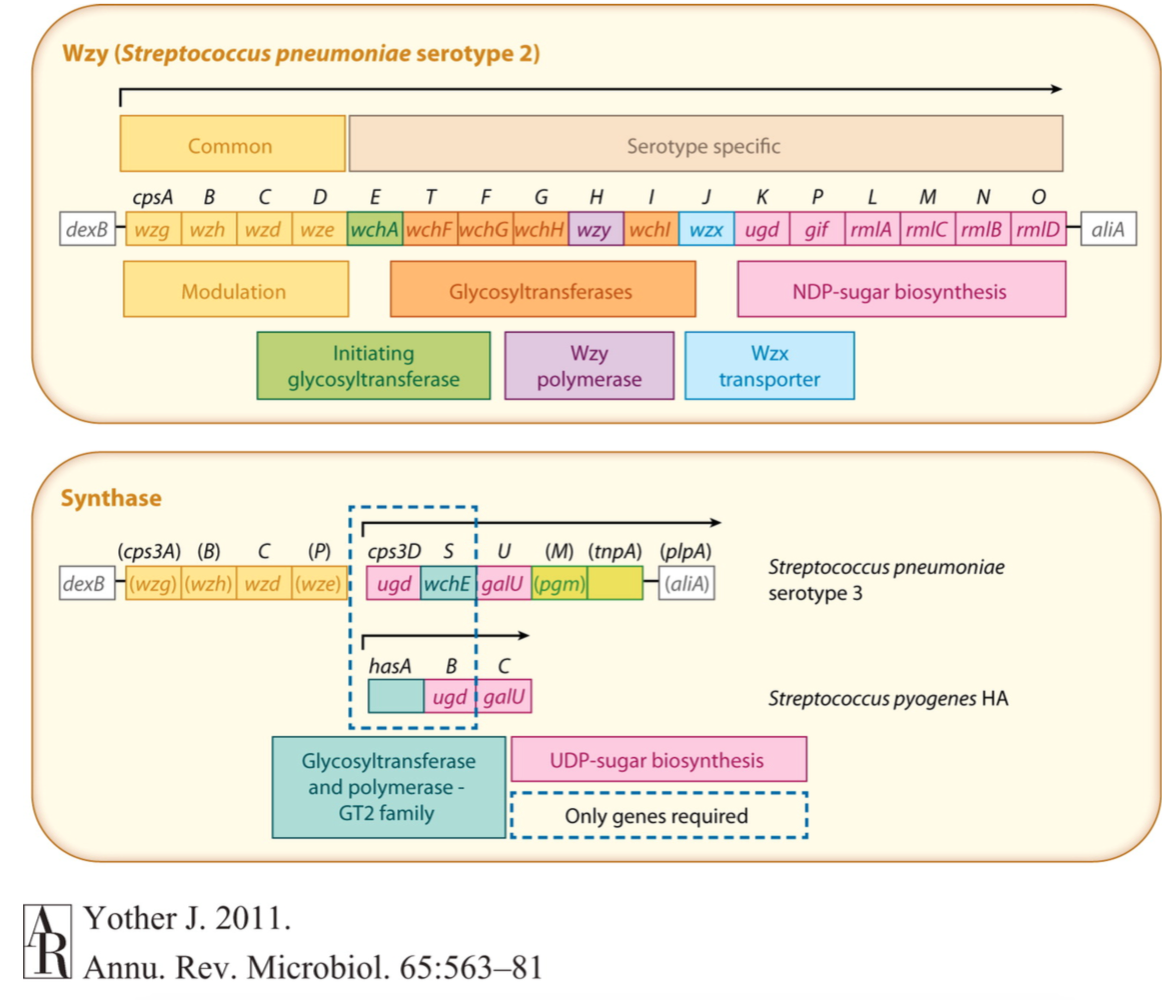
\includegraphics{img/cps_schema.png}
\caption{cps locus}
\end{figure}

    Traditionally, determining the serotype of \textit{S. pneumoniae} has
predominantly been done with the Quellung reaction or PCR, each with
their own limitations. Lately, focus has shifted towards serotyping
directly from genomic data.

    \hypertarget{seroba}{%
\subsection{SeroBA}\label{seroba}}

    Existing software to infer serotypes from genomic data are limited and
do not scale well. SeroBA is a pipeline that can quickly and accurately
determine the serotype of \textit{S. pneumoniae} from WGS data (Illumina
paired-end reads). It uses k-mer analysis and references to determine
the serotype of a sample.

In this tutorial we will walk you through how to determine the serotypes
of two samples using SeroBA, from setting up the necessary databases, to
running the analysis, and finally how to interpret the results.

For more information and to explore the code behind SeroBA, you can
visit the \href{https://github.com/sanger-pathogens/seroba}{GitHub
page}.

We will start with \href{db_setup.ipynb}{setting up the databases} with
a few simple commands. You can also \href{index.ipynb}{return to the
index}.


    % Add a bibliography block to the postdoc



\newpage






    \hypertarget{preparation-of-databases-before-running-seroba}{%
\section{Preparation of databases before running
SeroBA}\label{preparation-of-databases-before-running-seroba}}

    In order to use SeroBA for serotyping we must first download and prepare
the necessary databases. Start by moving into the data directory:

\begin{terminalinput}
\begin{Verbatim}[commandchars=\\\{\}]
\llap{\color{black}\LARGE\faKeyboardO\hspace{1em}} \PY{n+nb}{cd} data
\end{Verbatim}
\end{terminalinput}

    Now download the database from the GitHub repository:

\begin{terminalinput}
\begin{Verbatim}[commandchars=\\\{\}]
\llap{\color{black}\LARGE\faKeyboardO\hspace{1em}} svn checkout \PY{l+s+s2}{\PYZdq{}https://github.com/sanger\PYZhy{}pathog\PYZbs{}}
        \PY{l+s+s2}{    ens/seroba/trunk/database\PYZdq{}}
\end{Verbatim}
\end{terminalinput}

    \textbf{NOTE} if you are running a version of SeroBA older than v.0.1.3
the database is not packaged with the program and you will have to
download it using the below command instead:

\begin{verbatim}
seroba getPneumocat database_dir
\end{verbatim}

    KMC is used by SeroBA to count k-mers and ARIBA is used to avoid the
need for reads to be mapped to all reference sequences. Both of these
require a database to be set up.

To create a database for KMC and ARIBA run \textbf{createDBs}:

\begin{verbatim}
seroba createDBs database/ kmer_size
\end{verbatim}

Where the options are:

\begin{verbatim}
database       The database directory which you just downloaded
kmer_size      The k-mer size you want to use for kmc. Recommended = 71
\end{verbatim}

SeroBA uses a default k-mer size of 71 for a read length of 250 bp. When
deciding on a k-mer size, it is worth knowing that while a smaller k-mer
size can keep the memory requirements low, it will also reduce the
specificity. On the other hand, a larger k-mer size will require a
larger amount of memory but will produce more unique k-mers and thus
increase the specificity. What k-mer size to use also depends on the
read length.

\begin{terminalinput}
\begin{Verbatim}[commandchars=\\\{\}]
\llap{\color{black}\LARGE\faKeyboardO\hspace{1em}} seroba createDBs database/ 71
\end{Verbatim}
\end{terminalinput}

    If you are working with SeroBA on the Sanger farm, the database with
k-mer size 71 is already available centrally. This means you do not need
to create the database for using SeroBA on the Sanger farm.

However, for the sake of this tutorial, the above steps need to be
compleated before you can continue with the tutorial.

In the \href{run_seroba.ipynb}{next section} we are going to run SeroBA
to determine the serotype of one sample. You can also
\href{index.ipynb}{return to the index} or revisit the
\href{serotyping.ipynb}{previous section}.


    % Add a bibliography block to the postdoc



\newpage






    \hypertarget{running-seroba}{%
\section{Running SeroBA}\label{running-seroba}}

    We are now ready to use SeroBA to determine the serotype of our samples.
Move into the data directory where we keep the reads. In this case we
have called the directory \textbf{run\_seroba} and it is in the
directory called \textbf{data}.

\begin{terminalinput}
\begin{Verbatim}[commandchars=\\\{\}]
\llap{\color{black}\LARGE\faKeyboardO\hspace{1em}} \PY{n+nb}{cd} data/run\PYZus{}seroba
\end{Verbatim}
\end{terminalinput}

    Have a quick look at the contents of the directory:

\begin{terminalinput}
\begin{Verbatim}[commandchars=\\\{\}]
\llap{\color{black}\LARGE\faKeyboardO\hspace{1em}} ls \PYZhy{}al
\end{Verbatim}
\end{terminalinput}

    As you can see, there are two gzipped fastq files for each sample, one
for forward reads and one for reverse reads.

    Now run SeroBA using the \textbf{runSerotyping} command:

\begin{verbatim}
`seroba runSerotyping database forward_read reverse_read prefix`
\end{verbatim}

Where the options are:

\begin{verbatim}
database       path to the database directory
forward_read   forward read file in fastq format
reverse_read   reverse read file in fastq format
prefix         a unique prefix
\end{verbatim}

\begin{terminalinput}
\begin{Verbatim}[commandchars=\\\{\}]
\llap{\color{black}\LARGE\faKeyboardO\hspace{1em}} seroba runSerotyping ../database/ sample1\PYZus{}1.fq.gz \PY{l+s+se}{\PYZbs{}}
            sample1\PYZus{}2.fq.gz sample1
\end{Verbatim}
\end{terminalinput}

    If you are running Seroba on the Sanger farm and instead want to use the
central database, you can use:

\texttt{seroba\ runSerotyping\ \$SEROBA\_DB\ forward\_read\ reverse\_read\ prefix}

Lets have a look at the results in the \href{seroba_results.ipynb}{next
section}. You can also \href{index.ipynb}{return to the index} or
revisit the \href{db_setup.ipynb}{previous section}.


    % Add a bibliography block to the postdoc



\newpage






    \hypertarget{interpreting-the-results}{%
\section{Interpreting the results}\label{interpreting-the-results}}

    Now lets have a look at the results. Move into the data directory again.

\begin{terminalinput}
\begin{Verbatim}[commandchars=\\\{\}]
\llap{\color{black}\LARGE\faKeyboardO\hspace{1em}} \PY{n+nb}{cd} data/run\PYZus{}seroba
\end{Verbatim}
\end{terminalinput}

    Look at the file called \texttt{pred.tsv} in your results directoy,
\texttt{sample1}.

\begin{terminalinput}
\begin{Verbatim}[commandchars=\\\{\}]
\llap{\color{black}\LARGE\faKeyboardO\hspace{1em}} cat sample1/pred.tsv
\end{Verbatim}
\end{terminalinput}

    You can see three columns. The first one contains the prefix you chose
for the run. The second one contains the predicted serotype and the
third column may contain a comment regarding contamination. So, in this
case we can see that sample1 was predicted to be of serotype 8 and at
least 10\% of the reads are called as a different snp than the other
reads i.e.~there is contamination.

    Now, let's try again with the rest of the samples. All we need to do is
to run the runSerotyping option, but this time we will do it in a
for-loop so that we do not have to run the command manually for each
sample.

The command we are going to use will run \texttt{seroba\ runSerotyping}
on all fastq files in the working directory, so to avoid serytyping
sample1 again, first move the fastq files for this sample out from the
working directory:

\begin{terminalinput}
\begin{Verbatim}[commandchars=\\\{\}]
\llap{\color{black}\LARGE\faKeyboardO\hspace{1em}} mv sample1\PYZus{}* ../
\end{Verbatim}
\end{terminalinput}

    Run the command below. It will take around 10 minutes.

\begin{terminalinput}
\begin{Verbatim}[commandchars=\\\{\}]
\llap{\color{black}\LARGE\faKeyboardO\hspace{1em}} \PY{k}{for} file in *\PYZus{}1.fq.gz\PY{p}{;} \PY{k}{do} seroba runSerotyping \PY{l+s+se}{\PYZbs{}}
            ../database/ \PY{n+nv}{\PYZdl{}file} \PY{l+s+s2}{\PYZdq{}}\PY{l+s+si}{\PYZdl{}\PYZob{}}\PY{n+nv}{file}\PY{p}{//\PYZus{}1.fq.gz/\PYZus{}2.fq.gz}\PY{l+s+si}{\PYZcb{}}\PY{l+s+s2}{\PYZdq{}} \PY{l+s+se}{\PYZbs{}}
            \PY{l+s+s2}{\PYZdq{}}\PY{l+s+si}{\PYZdl{}\PYZob{}}\PY{n+nv}{file}\PY{p}{//\PYZus{}1.fq.gz/}\PY{l+s+si}{\PYZcb{}}\PY{l+s+s2}{\PYZdq{}}\PY{p}{;} \PY{k}{done}
\end{Verbatim}
\end{terminalinput}

    Now that we have performed multiple runs, we might want to create a
summary of the results. To do this, move up one level to the data
directory.

\begin{terminalinput}
\begin{Verbatim}[commandchars=\\\{\}]
\llap{\color{black}\LARGE\faKeyboardO\hspace{1em}} \PY{n+nb}{cd} ..
\end{Verbatim}
\end{terminalinput}

    Now run the \textbf{summary} option:

\begin{verbatim}
`seroba summary results_dir`
\end{verbatim}

Where the results\_dir in this case is \texttt{run\_seroba}.

\begin{terminalinput}
\begin{Verbatim}[commandchars=\\\{\}]
\llap{\color{black}\LARGE\faKeyboardO\hspace{1em}} seroba summary run\PYZus{}seroba
\end{Verbatim}
\end{terminalinput}

    Have a look at the resulting tsv file.

\begin{terminalinput}
\begin{Verbatim}[commandchars=\\\{\}]
\llap{\color{black}\LARGE\faKeyboardO\hspace{1em}} cat summary.tsv
\end{Verbatim}
\end{terminalinput}

    As you can see, you now have a summary of all the runs in one file. One
sample that might require some explanation is sample3 which was
serotyped as 6E(6B). Serogroup 6 is a bit different from the other
serogroups. The serotype of a sample can be 6E on the genotypic level,
and 6A or 6B on the phenotypic level. In this case, sample3 has the 6E
genotype and the 6B phenotype.

    Now follows some questions for you to go over what you have learned in
this tutorial one more time! You can find the answers in the link at the
bottom of the page.

\hypertarget{questions}{%
\section{Questions}\label{questions}}

\textbf{1. Your data requires you to use a kmer size of 60. You have
already downloaded the database to a directory called database\_60/.
What command would you run to create a database for KMC and ARIBA with
kmer size 60?}

\textbf{2. What is the predicted serotype of sample7?}

\textbf{3. How would you interpret the comment for sample7?}

This is the end of the tutorial. You can \href{index.ipynb}{return to
the index} or revisit the \href{run_seroba.ipynb}{previous section}.

The answers to the questions in this tutoial can be found
\href{Answers.ipynb}{here}.


    % Add a bibliography block to the postdoc



\end{document}
